\documentclass[11pt, a5paper, parskip=half-, DIV=12]{scrartcl}

\usepackage{../endeavour}
\usepackage{../endeavour_book}

\version{0.1}

\begin{document}
% Colour Cover
\thispagestyle{plain}
\AddToShipoutPictureBG{
\begin{tikzpicture}[remember picture, overlay]
	\node () at (current page.center) {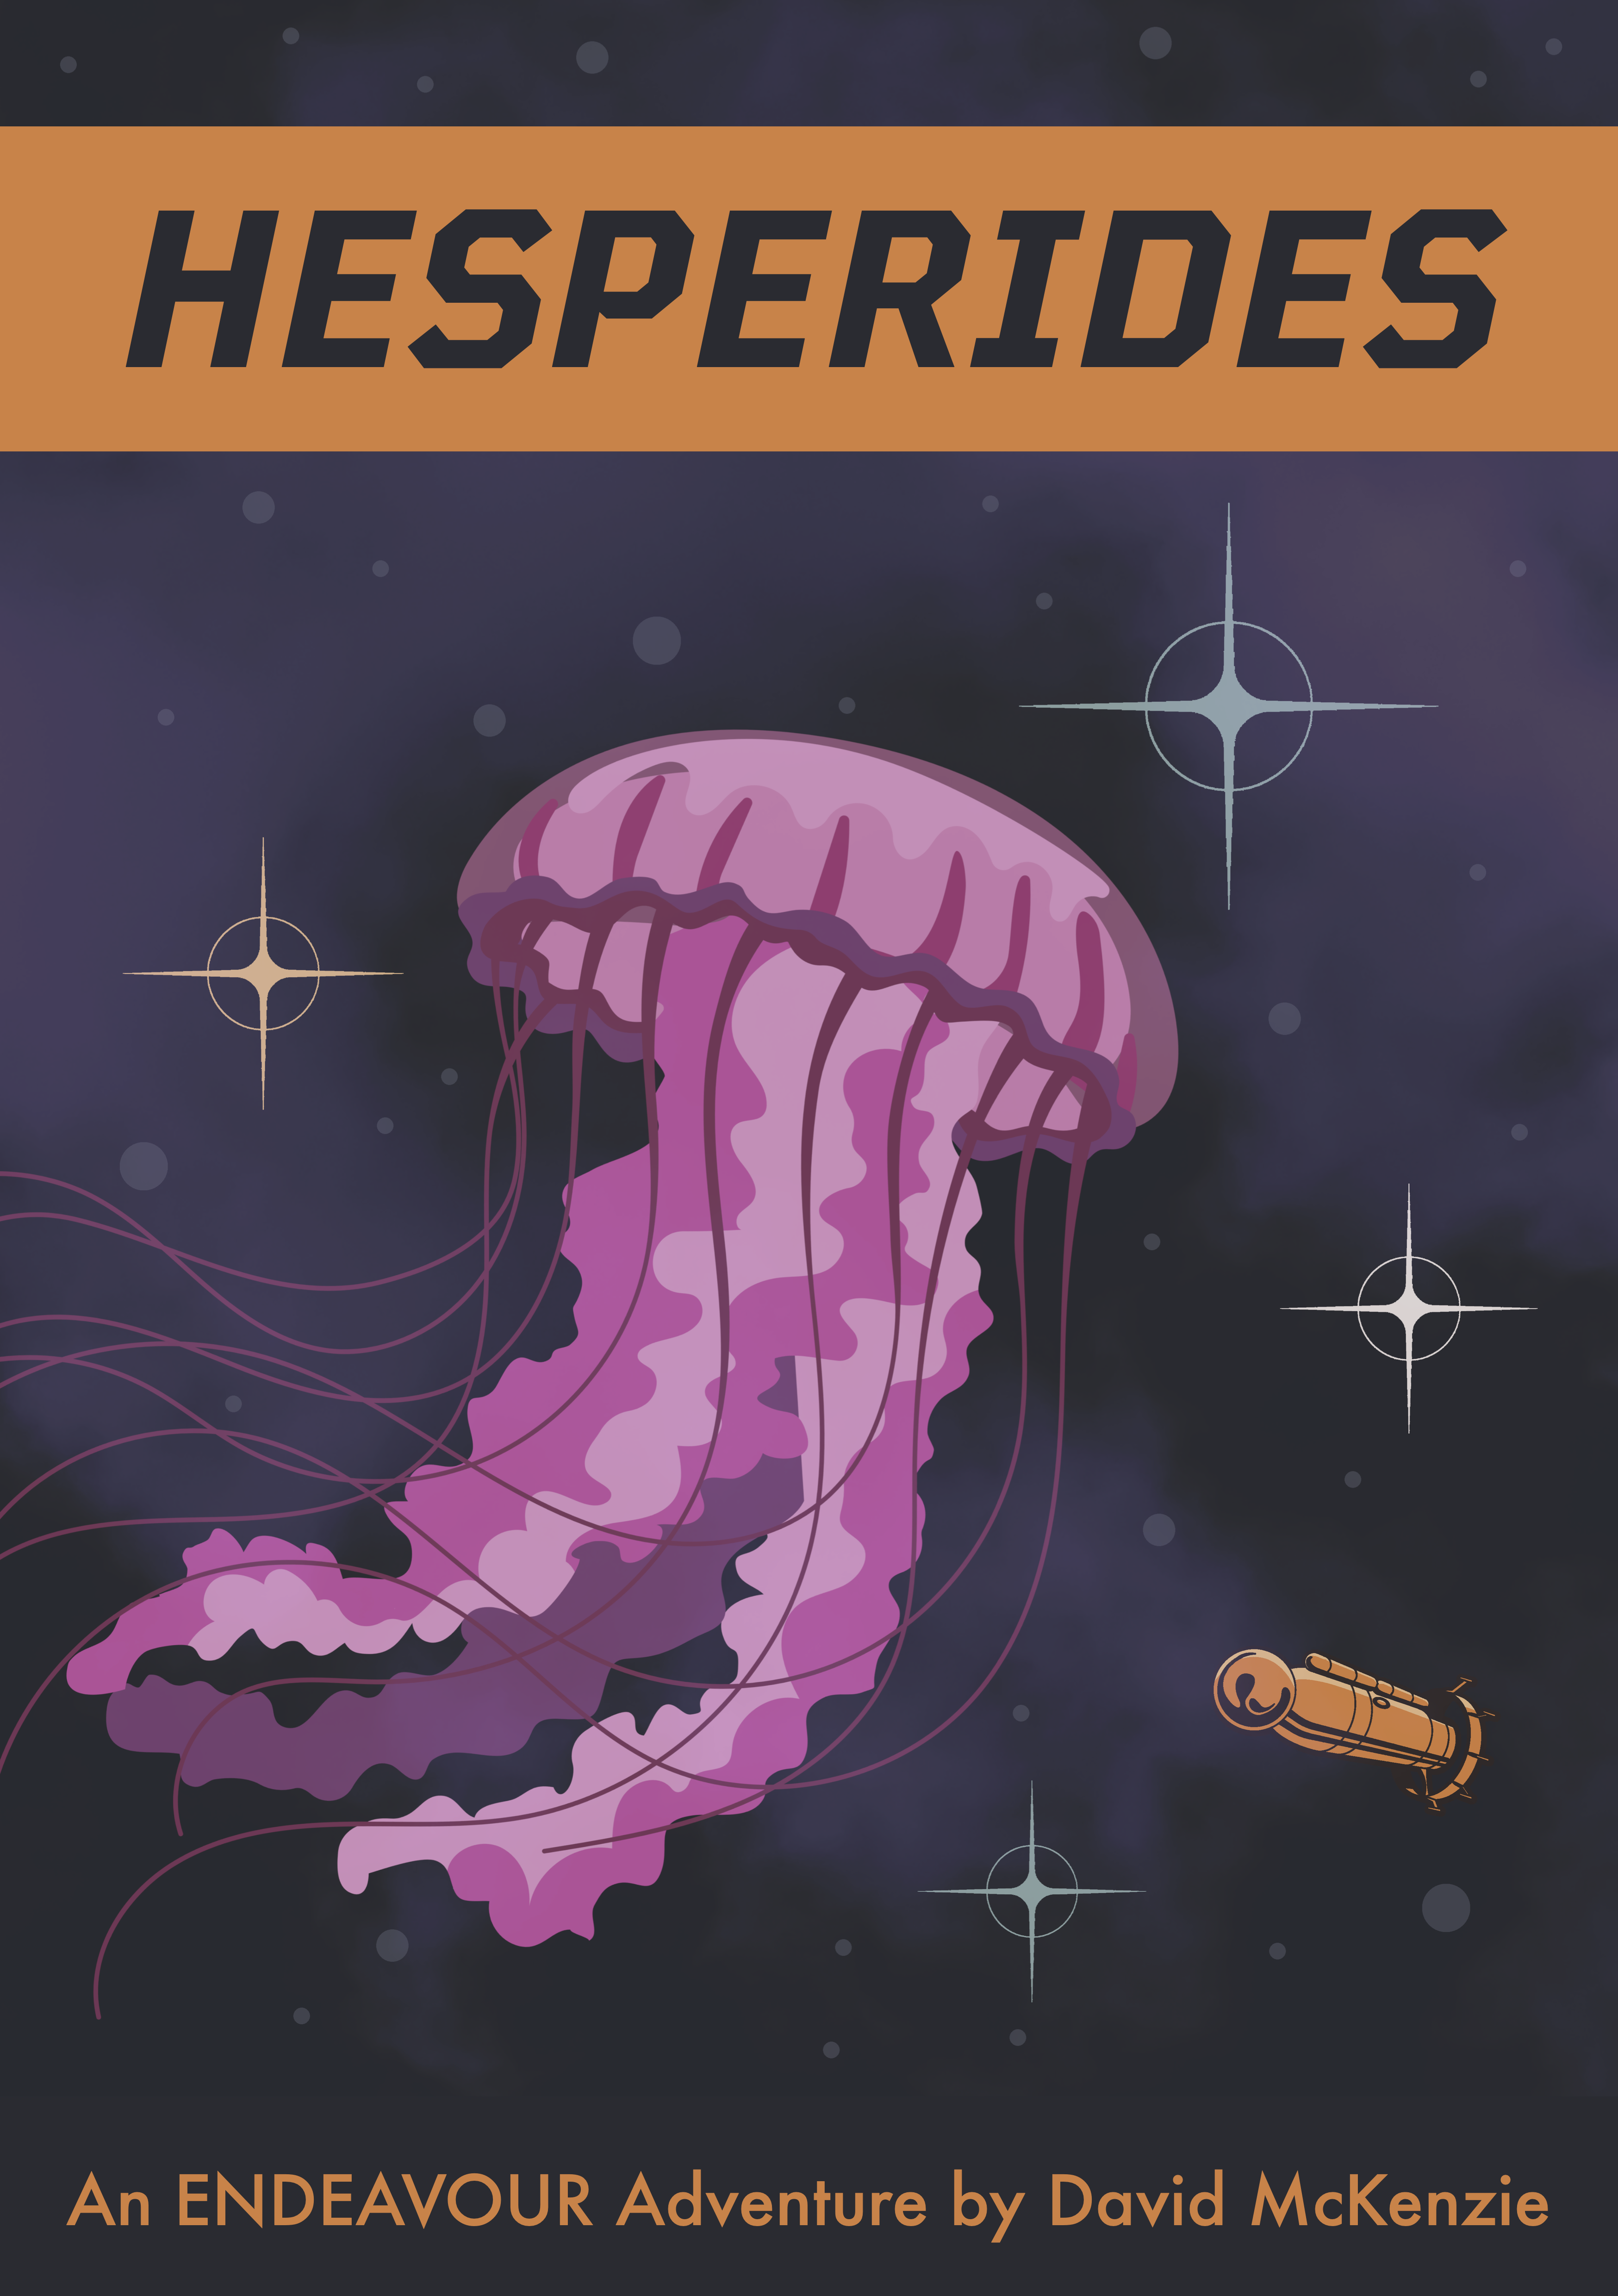
\includegraphics[width=\pagewidth, height=\pageheight]{Images/hesperides_cover.png}};
\end{tikzpicture}
}
{
\colorlet{headfootcolor}{LCARS_ORANGE}
\phantom{a}

\newpage
}

\ClearShipoutPicture
\AddToShipoutPictureBG{
	\begin{tikzpicture}[remember picture, overlay]
	\pic () at (current page.center) {starfield};
		\node[endeavour_box, minimum width=12.6cm, minimum height=18.8 cm] at (current page.center) {};
	\end{tikzpicture}
}

\setcounter{page}{1}
\setmainfont{TeX Gyre Schola}
\normalsize
\raggedright

\section*{Hesperides}
\textit{\textbf{Captain's Log:} Introduce the planet and any required exposition.}

\subsection*{Arrival}
A first challenge for the players to face.  This challenge should introduce the major theme of the adventure.

\subsubsection*{Challenge Name}
\begin{itemize}
	\item \textit{Will you \dots?} \textbf{Domain} vs. \textbf{Opponent}. \\ Additional details.
	\item \textit{Or will you \ldots?} \textbf{Domain} vs. \textbf{Opponent}. \\ Additional details.  
\end{itemize}

\newpage

\subsection*{Trials}
\subsubsection*{First Trial}
A situation that advances the story. \textit{Ask a leading question that suggests a possible challenge.} \textbf{Domain} vs. \textbf{Opponent}.

\subsubsection*{Second Trial}
A situation that advances the story. \textit{Ask a leading question that suggests a possible challenge.} \textbf{Domain} vs. \textbf{Opponent}.

\subsubsection*{Third Trial}
A situation that advances the story. \textit{Ask a leading question that suggests a possible challenge.} \textbf{Domain} vs. \textbf{Opponent}.

\subsection*{Crisis}

\begin{itemize}
	\item \textit{Will you \ldots?} \textbf{Threats:} Two or three threats.
	\item \textit{Or will you \ldots?} \textbf{Threats:} Two or three threats.
\end{itemize}

\newpage

\subsection*{Characters}
\begin{description}
	\item[Character Name (d?):] Epithet (d?), \ldots
	\item[Character Name (d?):] Epithet (d?), \ldots
	\item[Character Name (d?):] Epithet (d?), \ldots
\end{description}

\subsection*{Places}
\begin{description}
	\item[Place Name:] Brief description.
	\item[Place Name:] Brief description.
	\item[Place Name:] Brief description.
\end{description}

\subsection*{Mysteries}
\begin{description}
	\item[A fact about the planet.] \phantom{a} \\ A few related facts. \textit{One or two related questions.}
	\item[A fact about the planet.] \phantom{a} \\ A few related facts. \textit{One or two related questions.}
\end{description}

\newpage

\section*{Acknowlegements}
Much of the look and feel of \ENDEAVOUR{} is derived from its art, all of which was created by \textbf{svekloid}. This art was assembled from multiple collections available online at \href{http://shutterstock.com}{shutterstock.com} and then modified by Michael Purcell.  

\subsection*{Playtesters} \label{subsection:playtesters}
The following people helped to create \ENDEAVOUR{} by playing early versions of the game and providing invaluable feedback.\vspace{-1.75ex}
\begin{multicols}{2}
\begin{itemize}[noitemsep]
  \item Keydan Bruce
  \item Dannielle Harden
  \item Andrew Hellyer
%  \item Sarah Hewat
%  \item Scott Joblin
%  \item Sen-Foong Lim
  \item David McKenzie
%  \item Holly Moore
  \item Paul Murray
%  \item David Purcell
%  \item Heidi Purcell
  \item Kira Purcell
  \item Luke Purcell
  \item Meagan Purcell
%  \item Steve Purcell
%  \item Jason Stark
  \item Jo Stephenson
%  \item Pieter Vismans
  \item Brett Witty
  \item Bevis Worcester
  \item Evan Worcester
\end{itemize}
\end{multicols}

\subsection*{Design Tools} \label{subsection:design-tools}
The following tools were used to create this document:
\begin{description}[font=\normalfont\textbullet\space, noitemsep, topsep=-1ex]
	\item[LuaLaTeX:] Typesetting and layout.
	\item[TikZ:] Diagrams and art.
\end{description}
\vspace{1ex}
The fonts used are {\setmainfont{TT Mussels-BoldItalic} TT~Mussels~Bold~Italic},  \textsf{Futura}, and TeX~Gyre~Schola (cf. Century Schoolbook).

\vfill

\begin{tabular}{@{}m{7.775cm}@{\hspace*{0.375cm}}>{\centering\arraybackslash}m{2.6cm}@{}}
\textbf{Contact:} \href{mailto:endeavour.ttrpg@gmail.com}{endeavour.ttrpg@gmail.com}\newline \phantom{This is a test, only a test.} \newline \footnotesize{For use with the \textsc{Paragon} system, ©2020\newline \textbf{John Harper \& Sean Nittner}. \href{http://agon-rpg.com}{AGON-RPG.com}} & \includegraphics[scale=0.175]{Images/paragon_logo_mark.png} \\[5ex]
\footnotesize{This work is licensed under a Creative Commons \newline ``Attribution-ShareAlike 4.0 International'' license.} & \Huge{\doclicenseIcon}
\end{tabular}

\newpage

\thispagestyle{empty}

\tikzset{starfield/.pic={
	\node () at (current page.center) {
\includegraphics[width=\pagewidth, height=\pageheight]{Images/starfield.png}};
}}

\ClearShipoutPicture
\AddToShipoutPictureBG{
	\begin{tikzpicture}[remember picture, overlay]
	\pic () at (current page.center) {starfield};
	\end{tikzpicture}
}

\phantom{a}

\end{document}